\documentclass[tikz,border=10pt]{standalone}
\usepackage{amsmath,amssymb}
\usepackage{tikz}
\usepackage{pgfplots}
\pgfplotsset{compat=1.18}
\usetikzlibrary{arrows.meta,calc,patterns,positioning,shapes,decorations.markings,backgrounds,fit,intersections}

% Atlas colors
\definecolor{AtlasTeal}{HTML}{5BA4A4}
\definecolor{AtlasTealDark}{HTML}{4A8F8F}
\definecolor{AtlasTealLight}{HTML}{E8F4F4}
\definecolor{AtlasDeep}{HTML}{2C5F5F}
\definecolor{AtlasSage}{HTML}{7BAE7F}
\definecolor{AtlasSageLight}{HTML}{EDF5EE}
\definecolor{AtlasWarm}{HTML}{D4A853}
\definecolor{AtlasWarmLight}{HTML}{FDF6E8}

\begin{document}
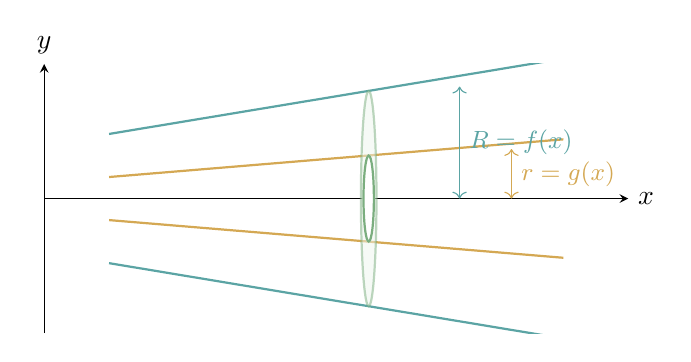
\begin{tikzpicture}
  \begin{axis}[
    width=9cm, height=5cm,
    axis lines=middle,
    xlabel={$x$}, ylabel={$y$},
    xtick=\empty, ytick=\empty,
    xmin=0, xmax=4.5, ymin=-2.5, ymax=2.5,
    every axis x label/.style={at={(ticklabel* cs:1)}, anchor=west},
    every axis y label/.style={at={(ticklabel* cs:1)}, anchor=south},
  ]
    % Outer curve (top)
    \addplot[AtlasTeal, thick, samples=80, domain=0.5:4] 
      {0.4*x + 1};
    \addplot[AtlasTeal, thick, samples=80, domain=0.5:4] 
      {-(0.4*x + 1)};
    % Inner curve (top)
    \addplot[AtlasWarm, thick, samples=80, domain=0.5:4] 
      {0.2*x + 0.3};
    \addplot[AtlasWarm, thick, samples=80, domain=0.5:4] 
      {-(0.2*x + 0.3)};
    % Washer at a cross-section
    \draw[AtlasSage, thick, fill=AtlasSageLight, opacity=0.5] 
      (axis cs:2.5,0) ellipse [x radius=0.06, y radius=2];
    \draw[white, thick, fill=white] 
      (axis cs:2.5,0) ellipse [x radius=0.04, y radius=0.8];
    \draw[AtlasSage, thick] 
      (axis cs:2.5,0) ellipse [x radius=0.04, y radius=0.8];
    % Labels
    \draw[<->, AtlasTeal] (axis cs:3.2,0) -- 
      node[right, font=\small] {$R=f(x)$} (axis cs:3.2,2.08);
    \draw[<->, AtlasWarm] (axis cs:3.6,0) -- 
      node[right, font=\small] {$r=g(x)$} (axis cs:3.6,0.92);
  \end{axis}
\end{tikzpicture}
\end{document}
